\documentclass{article}

\usepackage[T1]{fontenc}
\usepackage{polski}
\usepackage[utf8]{inputenc}

\usepackage{hyperref}
\usepackage[legalpaper, margin=0.8in]{geometry}

\usepackage{color}
\definecolor{deepblue}{rgb}{0,0,0.5}
\definecolor{deepred}{rgb}{0.6,0,0}
\definecolor{deepgreen}{rgb}{0,0.5,0}

\usepackage{listings}

% Python style for highlighting
\newcommand\pythonstyle{\lstset{
language=Python,
basicstyle=\ttm,
otherkeywords={self},             % Add keywords here
keywordstyle=\ttb\color{deepblue},
emph={MyClass,__init__},          % Custom highlighting
emphstyle=\ttb\color{deepred},    % Custom highlighting style
stringstyle=\color{deepgreen},
frame=tb,                         % Any extra options here
showstringspaces=false,            % 
basicstyle=\tiny
}}


% Python environment
\lstnewenvironment{python}[1][]
{
\pythonstyle
\lstset{#1}
}
{}

% Python for external files
\newcommand\pythonexternal[2][]{{
\pythonstyle
\lstinputlisting[#1]{#2}}}

% Python for inline
\newcommand\pythoninline[1]{{\pythonstyle\lstinline!#1!}}

\title{MISIO 2020 - Inteligentne Agenty}
\author{Bartosz Sobkowiak 125342}
\date{12.03.2020}

\usepackage{natbib}
\usepackage{graphicx}

\begin{document}

\maketitle
\section{Pytania}
\begin{enumerate}
    \item \textbf{Jakie cechy ma to środowisko?} \\
    Całkowicie obserwowalne, deterministyczne, epizodyczne, statyczne, dyskretne, jednoagentowe.
    
    \item \textbf{Jeden z agentów okazał się dużo lepszy. Dlaczego?} \\
    Drugi agent przestaje przemieszczać się lewo-prawo, jeśli oba pola są czyste. Wykonuje więc mniej ruchów (dostaje mniej punktów ujemnych), a osiąga taki sam efekt jak pierwszy agent, który cały czas sprawdza.
    
    \item \textbf{Czy agenty ReflexVacuumAgent lub ModelBasedVacuumAgent są racjonalne? Uzasadnij.} \\ 
    Agent pierwszy pomimo posiadania wiedzy dotyczącej stanu pól i tak się przemieszcza, więc nie maksymalizuje w ten sposób wartości miary jakości. Drugi agent stara się maksymalizować poprzez wykonywanie mniejszej liczby niepotrzebnych ruchów, lecz również nie jest racjonalny.
    
    \item \textbf{Czy dla tego środowiska istnieje racjonalny agent odruchowy? Uzasadnij.} \\
    Jeśli środowisko jest calkowicie obserwowalne, to agent odruchowy może być racjonalny (wykład, slajd 32). To środowisko jest obserwowalne, więc taki agent istnieje.
    
    \item \textbf{Jakie ma ono cechy?} \\
	Całkowicie obserwowalne, stochastyczne, epizodyczne, statyczne, dyskretne, jednoagentowe.

\end{enumerate}

\section{Kod agenta}
optilio: \textbf{bartek}
kod: \href{https://github.com/bbbrtk/misio_labs/tree/master/lab1}{github.com/bbbrtk/misio\_labs/lab1}

\pythonexternal{agent-code-only.py}

\section{Histogram}
Wartość oczekiwana: 44.3567 \\
Odchylenie standardowe: 19.0248 \\
Przedział ufności: (44.18990154342566, 44.52341845657433)
\begin{center}
    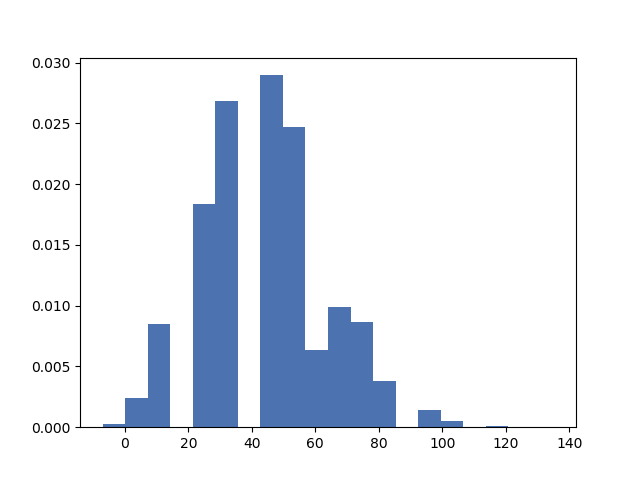
\includegraphics[width=0.5\textwidth]{chart.png}
\end{center}
\end{document}
